\documentclass[a4paper, 11pt]{article}

\usepackage[utf8x]{inputenc}
\usepackage[T1]{fontenc}
\usepackage{ucs}
\usepackage[english]{babel}
\usepackage{mathtools}
\usepackage{amsmath}
\usepackage{amsfonts}
\usepackage{ulem}
\usepackage{verbatim}
\usepackage{fancyhdr}
\usepackage[parfill]{parskip}
\usepackage{graphicx}
\usepackage{palatino}
\usepackage{float}
\usepackage[font={small,it}]{caption}

\linespread{1.05}
\pagestyle{fancyplain}
\fancyhead{}
\fancyfoot[L]{}
\fancyfoot[C]{}
\fancyfoot[R]{\thepage}
\renewcommand{\headrulewidth}{0pt}
\renewcommand{\footrulewidth}{0pt}
\setlength{\headheight}{13.6pt}

\widowpenalty=1000
\clubpenalty=1000

\newcommand{\horrule}[1]{\rule{\linewidth}{#1}}

\title{ 
\normalfont \normalsize 
\textsc{University of Copenhagen} \\ [25pt]
\horrule{0.5pt} \\[0.4cm]
\huge PCSD: Assignment 3 \\
\horrule{2pt} \\[0.5cm]
}

\author{Jens Fredskov (chw752)\\Henrik Bendt (gwk553)\\Ronni Lindsgaard (mxb392)} % Your name

\begin{document}
\maketitle
\pagebreak

\section{Recovery Concepts} % (fold)
\label{sec:recovery_concepts}

\subsection{} % (fold)

There is no need to implement a scheme for redo nor undo. As Force forces writes to disk for every write to memory, there is no need to ever redo an operation, as it is always commited. With No Steal means that dirty (uncommited) operations are never taken over by other operations, we never have to undo the opereration already written to disk.

% subsection  (end)

\subsection{} % (fold)

Non-volatile storage simply means, that when we cut off power, stored data is not lost (as opposed to volatile memory). This data can however be lost due to damages to disk like water damage, electrical overcharging (due to lightning strike), magnetic damage, mechanical damage (e.g. to write/read arm), error due to worn out hardware, etc.

Stable storage means that data stored is \textit{never} lost. This is a somewhat lose definition, as what does it mean to never lose stored data. If we assume that armageddon or a nuclear war is not around the corner, stable storage means that you do not lose data stored because of the above mentioned types of disk loss. This could be ensured by distributing data over a range of disks placed around the world (like clouding) in secured places and with lots of redundancy.

% subsection  (end)

\subsection{} % (fold)

\begin{enumerate}
    \item The log record for an update must be forced to disk before a data page for it gets written to disk 
    \item all log records for a transaction must be written to disk before a commit.
\end{enumerate}
Why do we need the above?
Lets assume data for an update/commit is written to disk, but the log is not forced to the stable storage.
\begin{enumerate}
    \item Then a crash occures and the log and main memory is lost. As the log was not written, we have no way of knowing that the write we just did to disk is not rightfully part of the comitted data and we cannot undo the incomplete actions. Thus we must ensure log is written before an update.
    \item  Then a crash occures in the middle of the commit and the log and main memory is lost. As the log was not written, we have no way of knowing what data on disk is dirty and also we must never forget comitted data. Thus we must ensure the log is written before a commit.
\end{enumerate}
These two protocols are sufficient, as the log explains all commits to the storage, so in principle we could do the log all over and reach the correct state of storage.

% subsection  (end)

% section recovery_concepts (end)

\section{ARIES} % (fold)
\label{sec:aries}

\begin{table}[H]
    \begin{minipage}{0.5\textwidth}
          \centering
  \begin{tabular}{|l|l|l|}
    \hline
    XID & Status & lastLSN \\
    \hline
    T1  & Running & 4 \\
    T2  & Running & 9 \\
    \hline
  \end{tabular}
  \caption{Xact table}
  \label{tab:xact}

    \end{minipage}
    \begin{minipage}{0.5\textwidth}
          \centering
  \begin{tabular}{|l|l|}
    \hline
    PID & recLSN \\
    \hline
    P2  & 3 \\
    P1  & 4 \\
    P5  & 8 \\
    P3  & 9 \\
    \hline
  \end{tabular}
  \caption{Dirty Page Table}
  \label{tab:dpt}

    \end{minipage}
\end{table}

\begin{enumerate}
    \item The transaction table and dirty page table can be seen in tables \ref{tab:xact}
and \ref{tab:dpt} respectively. \texttt{T3} is removed from the transaction
table as an \texttt{end} was found.
    \item The winner transactions are the ones completed, and the loser transactions
are the ones still in the transaction table. Hence $winners = \{T3\}$ and $losers =
\{T1,T2\}$.
    \item The redo phase starts at the log record where $LSN=3$ as this is the
record following the last checkpoint. The undo phase ends at the same log
record, as \texttt{TRAN\_ID} is one of the loser transactions.
    \item The log records that may cause page writes are records with
    $LSN \in \{3,4,8,9\}$ as all pages in
the table is written to by the loser transactions.
    \item The log records undone are the records with $LSN \in \{9,8,5,4,3\}$. The
    ToUndo set is initialised with \texttt{LSN}s $\{9,4\}$ from the transaction table and is
    expanded by checking the \texttt{LAST\_LSN} value of the record.
    \item The contents of the log is added with the lines visible in figure
    \ref{fig:clr}. The log semantics are changed such that for CLR records, the
    column \texttt{LAST\_LSN} points to the \texttt{LSN} of the record that was undone.
\end{enumerate}

\begin{figure}[h!]
  \centering
  \begin{minipage}{0.5\textwidth}
  \verbatiminput{misc/log_clr.txt}
  \end{minipage}
  \caption{Continuation of the log after crash recovery}
  \label{fig:clr}
\end{figure}


% section aries (end)

\section{Questions for Discussion on the Performance Measurements} % (fold)
\label{sec:questions_for_discussion_on_the_performance_measure_ments}

\subsection{} % (fold)

To generate the data in the bookstore we use the method \texttt{nextSetOfStockBooks} from \texttt{BookSetGenerator} to generate a set of 9001 books. All fields in the books generated from this are initialized using Javas \texttt{Random} class, except for \textit{salesMisses}, \textit{timesRated}, \textit{totalRating} which are always initialized as 0. All integers and strings are made from 32-bit integers (the strings are based of the id from the integer). All books starts out with between 1 and 10 copies.

The tests was all run on a Mac laptop, runnings OS X 10.8.5, with the following hard drive specification

\begin{table}[H]
\begin{tabular}{rl}
Capacity:           & 500.11 GB (500,107,862,016 bytes) \\ 
Model:              & APPLE HDD TOSHIBA MK5065GSXF      \\   
Rotational Rate:    & 5400                              \\   
Medium Type:        & Rotational                        \\   
Partition Map Type: & GPT (GUID Partition Table)        \\   
S.M.A.R.T. status:  & Verified                             
\end{tabular}
\end{table}

and 8 GB 1600 MHz DDR3 RAM and an Intel I5 Duo Core 2.5 GHz.

We have 2 runs for each iteration. We then have an iteration for every 5 workers from 5 to 50, meaning that we have 2 runs with 5 workers, 2 runs with 10 workers, and so forth. For each iteration we calculate the average and the standard deviation. We then plot the average of each iteration in a graph.

We decided to do all the runs on a single computer to get consistent results and avoid having the hardware influence the relation between the iterations. We have chosen the minimum number of workers to be 5 as each iteration is then increased by 5 giving a consistent increment. The maximum of 50 is arbitrary, but higher number of workers could pose a problem with regard to the time it takes running the experiment. The 2 number of runs for each iteration is arbitrary, but having multiple runs on each iteration allows us to calculate the average and standard deviation, thus adding to the credibility of the result. The hardware setup was chosen at random and is simply one of the computers we had at hand.

% subsection  (end)

\subsection{} % (fold)

\begin{figure}[H]
  \centering
  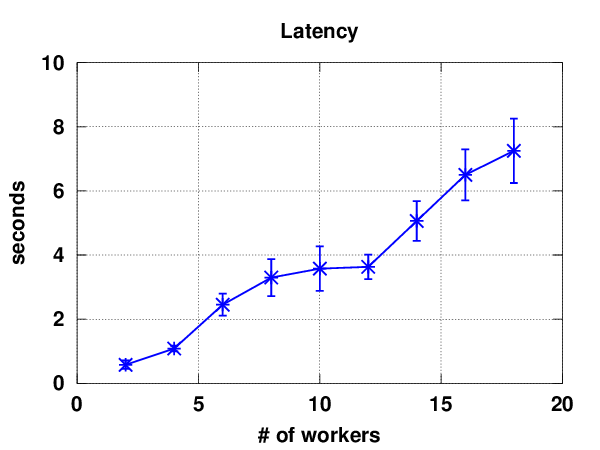
\includegraphics[width=0.85\textwidth]{images/latency.png}
  \caption{}
  \label{fig:latency}
\end{figure}

\begin{figure}[H]
  \centering
  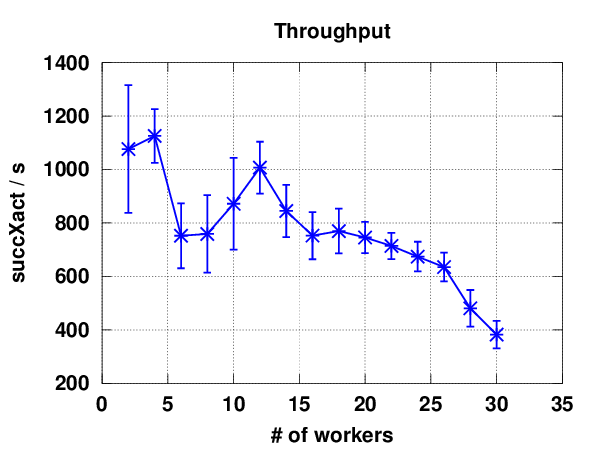
\includegraphics[width=1\textwidth]{images/throughput.png}
  \caption{}
  \label{fig:throughput}
\end{figure}


% subsection  (end)

\subsection{} % (fold)

%TODO Reliability of matrics and workload fo rpredicting performance
When the bookstore runs locally, as as a single process, it is not 
relevant to look at either of the other performance metrics besides throughput
and latency. The rest of the metrics are mostly relevant on networks and/or
threaded programs. This is also why latency increase linearly (by worker) when
running on a single core, which is not be the case for multi threaded programs.
e.g. the capacity of a single threaded bookstore is limited to server only one
request at a time, and would therefore be utilized 100 \% all the time.

For a multithreaded bookstore, capacity, utilization and scalability is
interesting to look at, as these figures are affected by the number of
concurrent requests the server can serve, as well as the number of clients
connecting to the service.

When testing the single process bookstore in a network environment it is also
interesting to test utilization and overhead as these figures could reveal
which bottlenecks are caused by the network and which are caused by the
application or server.

% subsection  (end)

% section questions_for_discussion_on_the_performance_measure_ments (end)

\end{document}
